\section{Introduction}

\frame
{
  \frametitle{Motivations}
%  \framesubtitle{Jean-Marc - 10 to 15 minutes}
\begin{block}{Scientific context}
\begin{itemize}
\item Potentially large size parallel applications.
\item Executing on large size parallel systems:\\
– Cluster and Grids \\
- Desktop grids\\
- P2P systems...
\end{itemize}
\end{block}
\begin{block}{Keypoints}
\begin{itemize}
\item Distributed heterogeneous resources
\item Dynamicity of the architecture
\item Scalability (huge amount of data)
\end{itemize}
\end{block}
%  \begin{itemize}
%  \item The institutions involved (UFRGS/UFSM/Grenoble/...)
%  \item The French-Brazilian collaboration in the domain
%  \item The importance of the visualization of parallel applications performance
%  \item The tutorial outline
%  \end{itemize}
}
\begin{frame}
\frametitle{Objective}
\begin{block}{Help users find performance errors:}
- Lack of parallelism, \\
- bottlenecks, overheads.\\
- Behavior analysis method
\end{block}
\begin{block}{Based on:}
- Execution model\\
- Measurement environment\\
- Visualisation model
\end{block}
\end{frame}

\begin{frame}
\frametitle{Representation of parallel program execution}
\begin{block}{Who ?}
\begin{itemize}
\item Program designer
\item Program certifier
\item Commercial selling parallel machines
\end{itemize}
\end{block}
\begin{block}{Why ?}
\begin{itemize}
\item Program debugging
\item Quantitative debugging (performance evaluation)
\item Dimensionning and performance tuning
\end{itemize}
\end{block}
\begin{block}{How ? }
\begin{itemize}
\item Graphical representation of the parallel execution
\item Interactive representation (exploration)\\
- zoom in and out on time, in the infrastructure, on objects\\
- compute statistics
\end{itemize}
\end{block}
\end{frame}
\begin{frame}
\frametitle{Methodology}
\begin{block}{Execution model}
\begin{itemize}
\item Abstraction of the parallel execution
\item Observability of states
\item Practical interest of states
\item Quality of observation (interaction tracer/application)
\end{itemize}
\end{block}
\begin{block}{Environment model}
\begin{itemize}
\item Structured set of resources (architecture)
\item Datation model
\item Manipulation language of states and events
\end{itemize}
\end{block}
\end{frame}
\begin{frame}

\frametitle{Collaboration (a not so short story)}
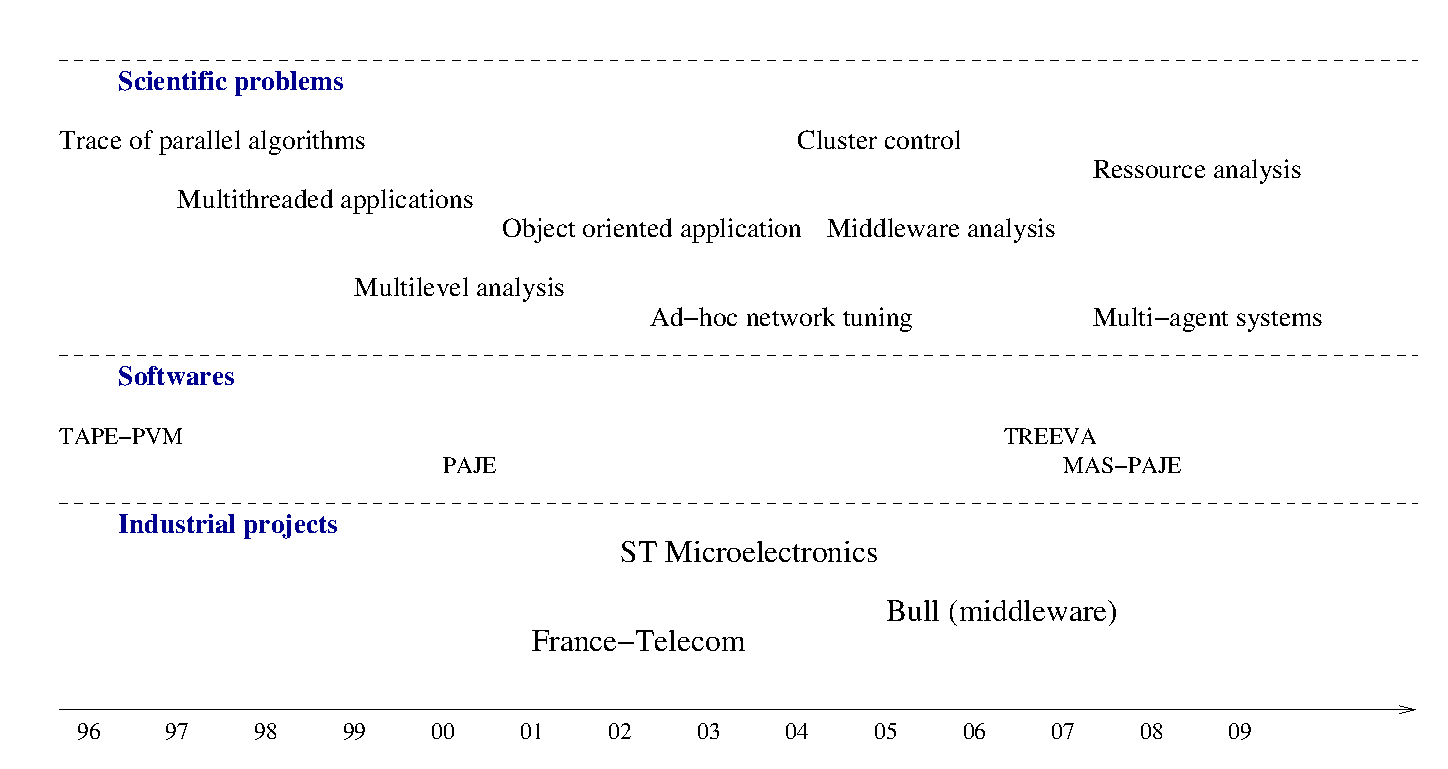
\includegraphics[width=1.1\textwidth]{img/collaboration.pdf}
\end{frame}


\begin{frame}
\frametitle{Tools for visualization}
State of the art

citer DeRose
\end{frame}

\begin{frame}
\frametitle{Main difficulties}
\begin{description}
\item Large scale
\item Dynamicity of the observed infrastructure
\item Coherence of views
\item Level of abstraction
\end{description}
\end{frame}

\begin{frame}
\frametitle{Typical examples (use case)}
\begin{description}
\item Multi-threaded application : un vieux (pierre-éric) ou un kaapi 
\item Resource usage monitoring : monitoring de grille 
\item Ad-hoc networks (distributed protocol) : travail de Corine
\item 
\item Object based distributed applications : multi-niveuau java
\item Multi-agent systems : exemple paams
\end{description}
\end{frame}
